\documentclass[english,12pt]{article}
%\usepackage[T1]{fontenc}
\usepackage[latin1]{inputenc}
%\usepackage{psfig}
\usepackage{graphics}
\usepackage{amsmath,amsthm,amssymb,babel}
\usepackage{color}
\renewcommand{\baselinestretch}{1.07}
\textwidth 6in \hoffset=-.4in \textheight=9.2in \voffset=-.9in
\parskip   1ex
\parsep    1ex
\itemsep   1ex
\vskip 5mm
\begin{document}
\vskip25mm
\section{Introduction}\label{S1}
The eye is the organ of vision; it allows the conversion of light into impulses in neurons. You can find a simple description its global structure below.\\
%\begin{center}
%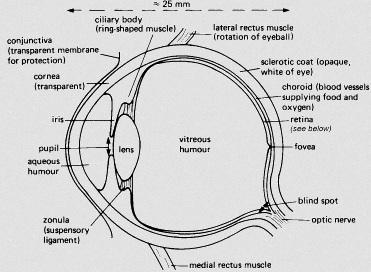
\includegraphics{Eye.jpg}\\
%\tiny{source:{http://academia.hixie.ch/bath/eye/home.html}}\\
%\small{Figure 1: Structure of the eye}
%\end{center}

\ Even now, the mechanisms who rule the functioning of the eye are not fully known because of the lack of data both in its mechanical and geometric characteristics. Therefore, some aspects of the behavior of the eye remain mysterious such as the elevated intraocular pressure, which is in fact a major risk factor for vision loss, that is to say glaucoma. Thus, a better understanding of the phenomena behind this so-called IOP becomes necessary.

\ In fact, glaucoma is a multi-factorial eye disease which means it is not exactly caused by an elevated IOP. In other words, there is no specific level of IOP that definitely leads to glaucoma! However, because of our lack of knowledge, this is the only factor we can act on. 

\ For now, there exist several medications such as carbonic anhydrase inhibitors or beta-blockers that 
should lower of the IOP. Unfortunately, the response to this medications is not consistent among patients since some physiological factors are assumed to influence the drug efficacy. Because the determining factors can only be deduced from clinical data, that is to say in vivo, they are quite difficult to isolate. Among the suspects, there are: the blood pressure, the levels of IOP itself, the gender, the ethnic group...And there is no end to it. By analysing the clinical data on a really significant number of patients, it would give us some way toward answering this question, which is still under investigation. Several studies have already been carried out on this subject. Here, we choose to build a mathematical model of intraoccular fluid dynamics instead. 

\ The rest of the paper is structured as follows. In Section 2, we present some medical aspects about the structure of the eye and the glaucoma. In Section 3, we describe the model of intraocular fluid dynamics. And, finally, in section 4 we present numerical simulations.

\section{Medical aspect}\label{s2}
\subsection{Description of the eye}
\subsubsection{Aqueous humor }\
\indent\ Our main interest resides in the flow of aqueous humor, which is a transparent, gelatinous fluid similar to plasma located in the anterior and posterior chambers of the eye. Aqueous humor is produced by the ciliary epithelium and drains into the Schlemm's canal. The balance between production and drainage of aqueous humor regulates the fluid pressure inside the eye, also known as intraocular pressure (or IOP). \\
%\begin{center}
%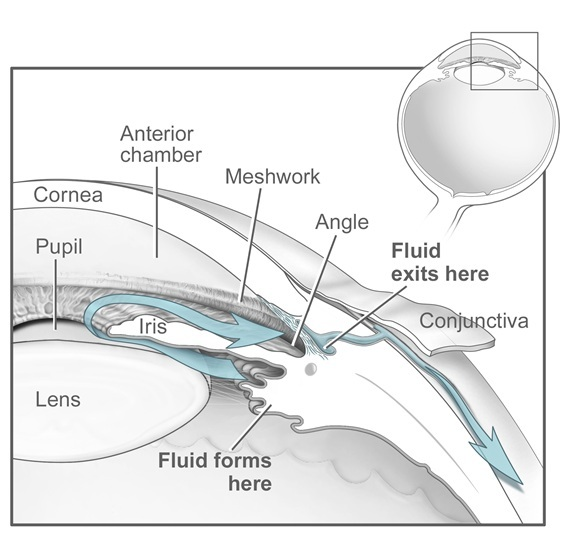
\includegraphics{Humor.jpg}\\
%\small{Figure 2: Flow of the aqueous humor}
%\end{center}
\indent In healthy individuals, IOP ranges between 10 and 22 mmHg, with an average value of 16. 
IOP inflates the eye globe and help maintaining its almost spherical shape, which is very important for a correct vision. 
IOP can be measured experimentally by tonometry as depicted in the figure below.\\
%\begin{center}
%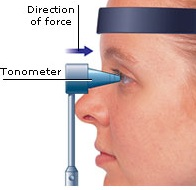
\includegraphics{Tonometry.jpg}\\
%\tiny{source:{http://www.aviva.co.uk/health-insurance/home-of-health/medical-centre/medical-encyclopedia/entry/test-tonometry/}}
%\small{Figure 3: Tonometer}
%\end{center}
\indent The ophthalmologist uses a fine jet of air directed toward the cornea and the machine measures the pressure by looking at the deformation when the air hits the eye. This measure is corrected by an algorithm that takes into account the thickness of the cornea, otherwise the value of IOP might be underestimated/overestimated.
Problems begin with an elevated IOP which is a major risk factor for vision loss.

\subsubsection{Glaucoma}\
\indent Glaucoma, also called the silent thief of sight, is the second leading cause of blindness worldwide (1 in 40 adults over 40 years old). This disease can be described as a group of ocular disorders with multi-factorial etiology united by a clinically characteristic optic neuropathy accompanied by a vision loss. Even though the exact origin of glaucoma is not known yet, there are two kinds of diagnostics: morphological damages and physiological/functional damages.\\
As shown in the figure below, the morphological diagnostic is based on detecting alterations in the shape of the optic nerve head (ONH), which is the part of the optic nerve that enters the eye.
%\begin{center}
%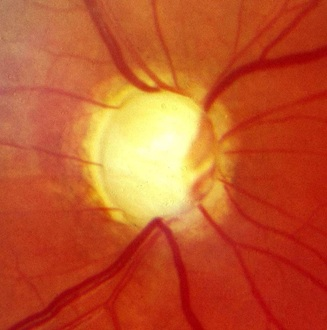
\includegraphics{Morphological.jpg}\\
%\small{Figure 4: Glaucomateous optic nervehead demonstrating increased cup to disc ratio}
%\end{center}
 More precisely, to estimate the degree of gravity of morphological changes in the ONH, we use the following formula:
$$ R=\frac{Area\ of\ the\ excavated\ surface}{Area\ of\ the\ whole\ ONH}$$
If $R>0.4$, in the general case, it is reasonable to assume that the patient suffers from glaucoma.\\

Nevertheless, the size of the optic nerve head must be taken into account since the most important part is the area of the non excavated surface. As a matter of fact, if the ONH of a patient is very large (diameter) even with $R=0.5$ he may never contracts glaucoma; the alterations in the shape of the ONH are harmless. Conversely if the ONH is small, even with $R=0.2$, our patient is likely to contract glaucoma.\\

Physiological/functional diagnostic in glaucoma is based on the loss of visual field, which is the total area in which you can see objects while you focus your eyes on a central point.\\
%\begin{center}
%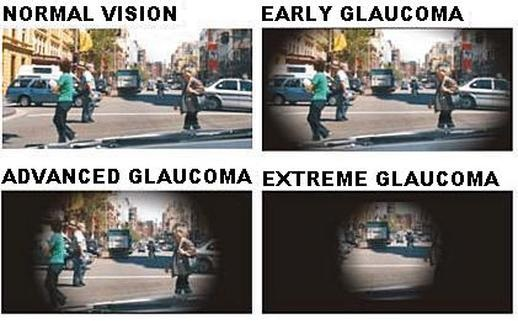
\includegraphics{Glaucoma.jpg}\\
%\tiny{source:{http://www.swisscompleteeyecare.com/uploads/3/6/3/8/3638142/8901258.jpg?520}}\\
%\small{Figure 5: Evolution of the vision field for a Glaucoma patient}
%\end{center}
In healthy individuals, the visual field can be described with the following angles:\\
-50 to 60 degrees superiorly\\
-70 to 75 degrees inferiorly\\
-60 degrees nasally\\
-90 to 100 degrees temporally\\

As the glaucoma progresses, these angles will decrease. Unfortunately, the damage to the optic nerve in glaucoma is irreversible. Thus, the only treatments now available for glaucoma patients aim at preventing further damage to the optic nerve, but the lost vision cannot be regained.\\
%
\indent Elevated IOP is a major risk factor for glaucoma and, in fact, it is the only treatable factor in glaucoma, even though it is neither a necessary nor a sufficient condition for glaucomatous damage. Indeed, a patient could have a glaucoma but low IOP (condition also called normal tension glaucoma), whereas a patient with an elevated IOP (condition also called ocular hypertension) may never develop glaucoma. However, the IOP remains the only parameter we can act on, either by surgery or with medications. 
Unfortunately, 25 \% of IOP-treated patient progress to blindness and there is nothing we can do about it with our current knowledge.
\subsection{IOP-lowering medications}
\subsubsection{List of medications}
IOP-lowering medications have two effects: either decrease the secretion of aqueous humor by the ciliary epithelium or increase its elimination through the Schlemm's canal. It is also possible to combine secretion/elimination treatments in order to decrease IOP even more.

Here is a list of the medications commonly used:\\
\begin{tabular}{|c|c|}
\hline
Decrease the secretion of aqueous humor & Increase the elimination of aqueous humor\\
\hline
beta-adrenergic receptor antagonists & Prostaglandin analogs \\
Alpha2-adrenergic agonists & Miotic agents \\
alpha agonists &  \\
Carbonic anhydrase inhibitors &  \\
\hline
\end{tabular}
\subsubsection{Different effects on patients}\
\indent Note that certain drugs could work better on patients depending on their age, gender, ethnic group, localization, other diseases like diabetes, hypertension ...There are too many unknown factors to take into account, since each patient reacts differently. 
Consequently, it is currently very difficult to predict how a specific patient will respond to different IOP-lowering medications, posing serious challenges to the choice of best clinical management of glaucoma patients.\\

Several clinical/statistical studies have already been carried out on these questions and brought interesting results. However, due to the complexity of the system, many of the phenomena regulating the build-up of IOP remain poorly understood. Thus, in this work we contribute to this research field by using a mathematical model to theoretically investigate the influence of different IOP-lowering mechanisms on individuals presenting different systemic conditions.
 
\section{The model}\label{s3}\
\indent Our aim is to understand the link between IOP, secretion and elimination of aqueous humor and arterial blood pressure.
Because of the lack of data about the geometry and the characteristics of the eye, we chose to present a general model rather than a detailed study of the fluid flow. Such a simple model will be useful to analyze different hypotheses about these processes.
\subsection{Formulation of the problem}\
\indent The eye is modeled as a shell filled with liquids and containing solid structures. 
 The total aqueous humor volume $U$, 
 the fluid inflow in posterior chamber $F_h$ and
 the net outflow via trabecular path $F_e$ are linked by the simple balance equation:
\begin{equation}
\frac{dU}{dt}=F_{h}-F_{e}\,.
\label{e1}
\end{equation}
\\
\textbf{Outflow process}\\
We assume that the pressure in both chambers is equal to the intra-ocular pressure $p$ and that the outflow is regulated by a hydrostatic pressure difference, resulting in the following hydraulic equivalent of Ohm's law:
\begin{equation}
F_{e}= \frac{p-p_{e}}{R}
\label{e2}
\end{equation}
with
\begin{itemize}
\item $p_e$: pressure in the episcleral veins (here taken as a given output pressure)
\item $R$: output resistance
\end{itemize}
\textbf{Inflow process}\\
The intraocular fluid and the solutes in it come from the blood in the capillaries. However, there exist several layers between the capillary blood and the intraocular fluid, and each layer is permeable to different solutes. 

Thus, we consider here an equivalent membrane which is impermeable to large protein molecules and semipermeable to low molecular components. Therefore, $L_p$ is equivalent to the inverse of a resistance. The fluid moves through the membrane because of a combination of hydrostatic and osmotic pressure differences between blood and aqueous humor.\\
The fluid inflow is then described by the following equation:
\begin{equation}
F_{h}= L_p \big[ (p_a-p)-\sigma_{p} \Delta\pi_{p}-\sigma_{s} \Delta\pi_{s}\big]
\label{e3}
\end{equation}
with
\begin{itemize}
\item $L_p$: permeability of the equivalent membrane
\item $p_a$: pressure in the ciliary body capillaries
\item $p$: IOP
\item $\sigma_p$: reflection coefficient (proteins)
\item $\sigma_s$: reflection coefficient (low molecular components)
\item $\Delta \pi_p $: osmotic pressure difference accross membrane (proteins)
\item $\Delta \pi_s $: osmotic pressure difference across membrane (low molecular component)
\end{itemize}
Here, $\Delta \pi_p $ is assumed to depend only of the concentration of the proteins in the arterial blood (almost no blood protein in the aqueous humor and implies that $\sigma_p=1$) while and $\Delta \pi_s $ is proportional to the difference of the total molar concentration of the low molecular components across the membrane.
\begin{equation}
\Delta\pi_{s}= \rho(C_1-C_{2})
\label{e4}
\end{equation}

\textcolor{red}{GG: I ARRIVED TILL HERE!}

With
\begin{itemize}
\item $\rho$: universal gas constant $\times$  absolute temperature
\item $C_1$: total molar concentration of low-molecular components (blood)
\item $C_2$: total molar concentration of low-molecular components (intra-ocular fluid near ciliary body surface)
\end{itemize}
If theses concentrations are small enough, the flux of the low-molecular solutes across the membrane is determined by (\ref{e5}), the sum of the diffusive, convective and active components
\begin{equation}
Q_s=\xi_s(C_1-C_{2})+F_h (1-\sigma_s) \bar{C}+J
\label{e5}
\end{equation}
With
\begin{itemize}
\item $\xi_s$: average permeability of the membrane for the low molecular species
\item $\bar{C}=\frac{C_1+C_2}{2}$
\item $J$: influx due to the active transport
\end{itemize}
At this point, in order to obtain the equation of the solute mass balance (\ref{e6}), several considerations must be introduced:\\
$\textbf{1)}$Normally, $Q_s$ only contributes to the composition of the intraocular fluid; the solid structures have their own part to play. We should have taken into account the transport and transfer processes on all the flow segments to describe correctly the solute transport. Fortunately, (\ref{e2}) implicitly shows that there is no osmotic effect for the outflow meaning that the concentration level doesn't matter for the outflow.\\
$\textbf{2)}$ Let $V^{\ast}$ be the volume of intraocular fluid between the folds of the ciliary body. If $T_1$ is the characteristic time of diffusing in this region, if $T_2$ is the dwell time of the fluid in this region ($T_1<<T_2$, from anatomical data) and if the characteristic time of the problem is greater than $T_1$ then the concentration at the input/output can be considered equal to the average concentration in $V^{\ast}$.\\
$\textbf{3)}$ From anatomical data, since the dwell time of the fluid in the posterior chamber $T_3$ is two orders lower than the diffusion time $T_4$, we can neglect the diffusion phenomena in favour of the convection for $Q_e$, the solute outflow from $V^{\ast}$ into the posterior chamber.\\
$\textbf{4)}$ From anatomical data, we find that the transmembrane diffusion in (\ref{e5}) can also be neglected as compared with convection.\\

Then:
\begin{equation}
V^{\ast} \frac{dC_{2}}{dt}= Q_s-Q_e=F_h (1-\sigma_s) \bar{C}+J-F_h C_2
\label{e6}
\end{equation}
Let $V$ be the volume of the eye. If we assume that the volume of the solid structure and the volume of the vitreous humor is constant ant that the volume of the blood in the blood vessels can be time-averaged for slow processes
\begin{equation}
dV = dU
\label{e7}
\end{equation}
Finally, we combine (\ref{e1})-(\ref{e7}) to obtain the formulation of the problem
\begin{equation}\label{e8}
\left\{\begin{array}{ll}
\displaystyle{\frac{dV}{dt}}= L_p \big[ (p_a-p)-\Delta\pi_{p}-\sigma_{s} \Delta\pi_{s}\big]-\frac{p-p_{e}}{R},\quad \Delta\pi_{s}=\rho(C_1-C_{2})\\
\quad V^{\ast} \displaystyle{\frac{dC_{2}}{dt}}=J+L_p\big[(p_a-p)- \Delta\pi_{p}-\sigma_{s} \Delta\pi_{s}\big] \big[(1-\sigma_s)\displaystyle{\frac{C_1+C_2}{2}-C_2\big]}
\end{array}\right.
\end{equation}

\subsection{Stationary case}
Since $V$ does not vary with time, the inflow rate is equal to the outflow rate:
\begin{equation}\label{e9}
\left\{\begin{array}{ll}
L_p \big[ (p_a-p)- \Delta\pi_{p}-\sigma_{s} \Delta\pi_{s}\big]=\displaystyle{\frac{p-p_{e}}{R}}, \quad \Delta\pi_{s}=\rho(C_1-C_{2})\\
\qquad\qquad F_h (1-\sigma_s) \bar{C}+J=F_h C_2, \quad\overline{C}= \displaystyle{\frac{C_1+C_2}{2}}
\end{array}\right.
\end{equation}
Our aim is to study the influence of $R$ on the hydrodynamic characteristics of the system, that is $F_h$ and $p$. Therefore, we fix the parameters of the membrane and the blood state and consider (\ref{e9}) for 2 simple flow regimes:\\
-$1$: Purely hydraulic model ($\Delta\pi_s$ is constant)\\
-$2$: Osmotic components dynamics ($J$ is constant)\\
In this case, the system (\ref{e9}) can be solved easily
\begin{equation}\label{e10}
\left\{\begin{array}{ll}
p=\displaystyle{\frac{R L_p(p_a-\Delta\pi_{p}-\sigma_{s} \Delta\pi_{s})+p_e}{R L_p+1}}\\
F_h=F_e=\displaystyle{\frac{L_p}{R L_p +1}}(p_a-\Delta\pi_{p}-\sigma_{s} \Delta\pi_{s}-p_e)\\
\Delta\pi_{s}=\rho(C_1-C_{2})
\end{array}\right.
\end{equation}
And we have
%\begin{center}
%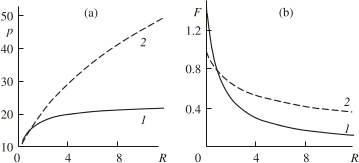
\includegraphics{courbes_pr_fr.png}\\
%\tiny{source :{Dynamic of the intraocular fluid}Lyobimov et al, 2007}\\
%\small{Figure 6: $IOP$ and $F_h$ in the stationary case}
%\end{center}
\subsection{Nonstationary case}
First, a relationship between $V$ and $p$ is needed.\\
Given the elasticity properties of the eye shell and assuming small pressure deviations from a certain $p_0$, we can linearize $V$.
\begin{equation}
V = V(p) \approx V_0 + \alpha (p-p_0)
\end{equation}
where $\alpha$ is the volume compliance of the eye shell (note that this value may vary from one patient to another).\\
The system (\ref{e8}) is replaced by
\begin{equation}\label{e11}
\left\{\begin{array}{ll}
 \alpha \displaystyle{\frac{dp}{dt}}=F_{h}-\displaystyle{\frac{p-p_e}{R}}\\
V^{\ast} \displaystyle{\frac{dC_{2}}{dt}}= F_h(1-\sigma_s)\overline{C} + J - F_hC_2,\; \overline{C}= \frac{C_1+C_2}{2}
\end{array}\right.
\end{equation}

\subsection{Numerical results}
We used equation \eqref{e9} to obtain first non-stationary numerical result using \texttt{Octave} function \texttt{ode45}, that solve equation with the well known explicit Runge–Kutta method of order (4,5).  The point here was to make a first step to a better understanding of the roles of the different parameters of our equation that seem of interest to us, \textit{i.e.} the resistance $R$ and the permeability $L_p$. We also aim at comparing the behaviour of IOP on different patient profile. 


For sake of simplicity we focus on patient arterial pressure. We consider three arterial pressure profile : a low arterial blood pressure  (LBP) of $26.6$, a normal arterial blood pressure (NBP) of $31.1$, and a high blood arterial pressure (HBP) of $35.5$.

We take physiological datas from the literature \textcolor{red}{INSERER CITATION Lyubimov et al, 2007,Anders, 1975,The mechanism of aqueous humour
formation,2002 \cite{•}}, and our initial values in physiological range. As it is a first step to simulation, we decide to neglect here the oscillating component. 

\begin{figure}[htbp]
 \centering
  \subfigure[Time evolution of IOP\label{fig:IOPt}]{
    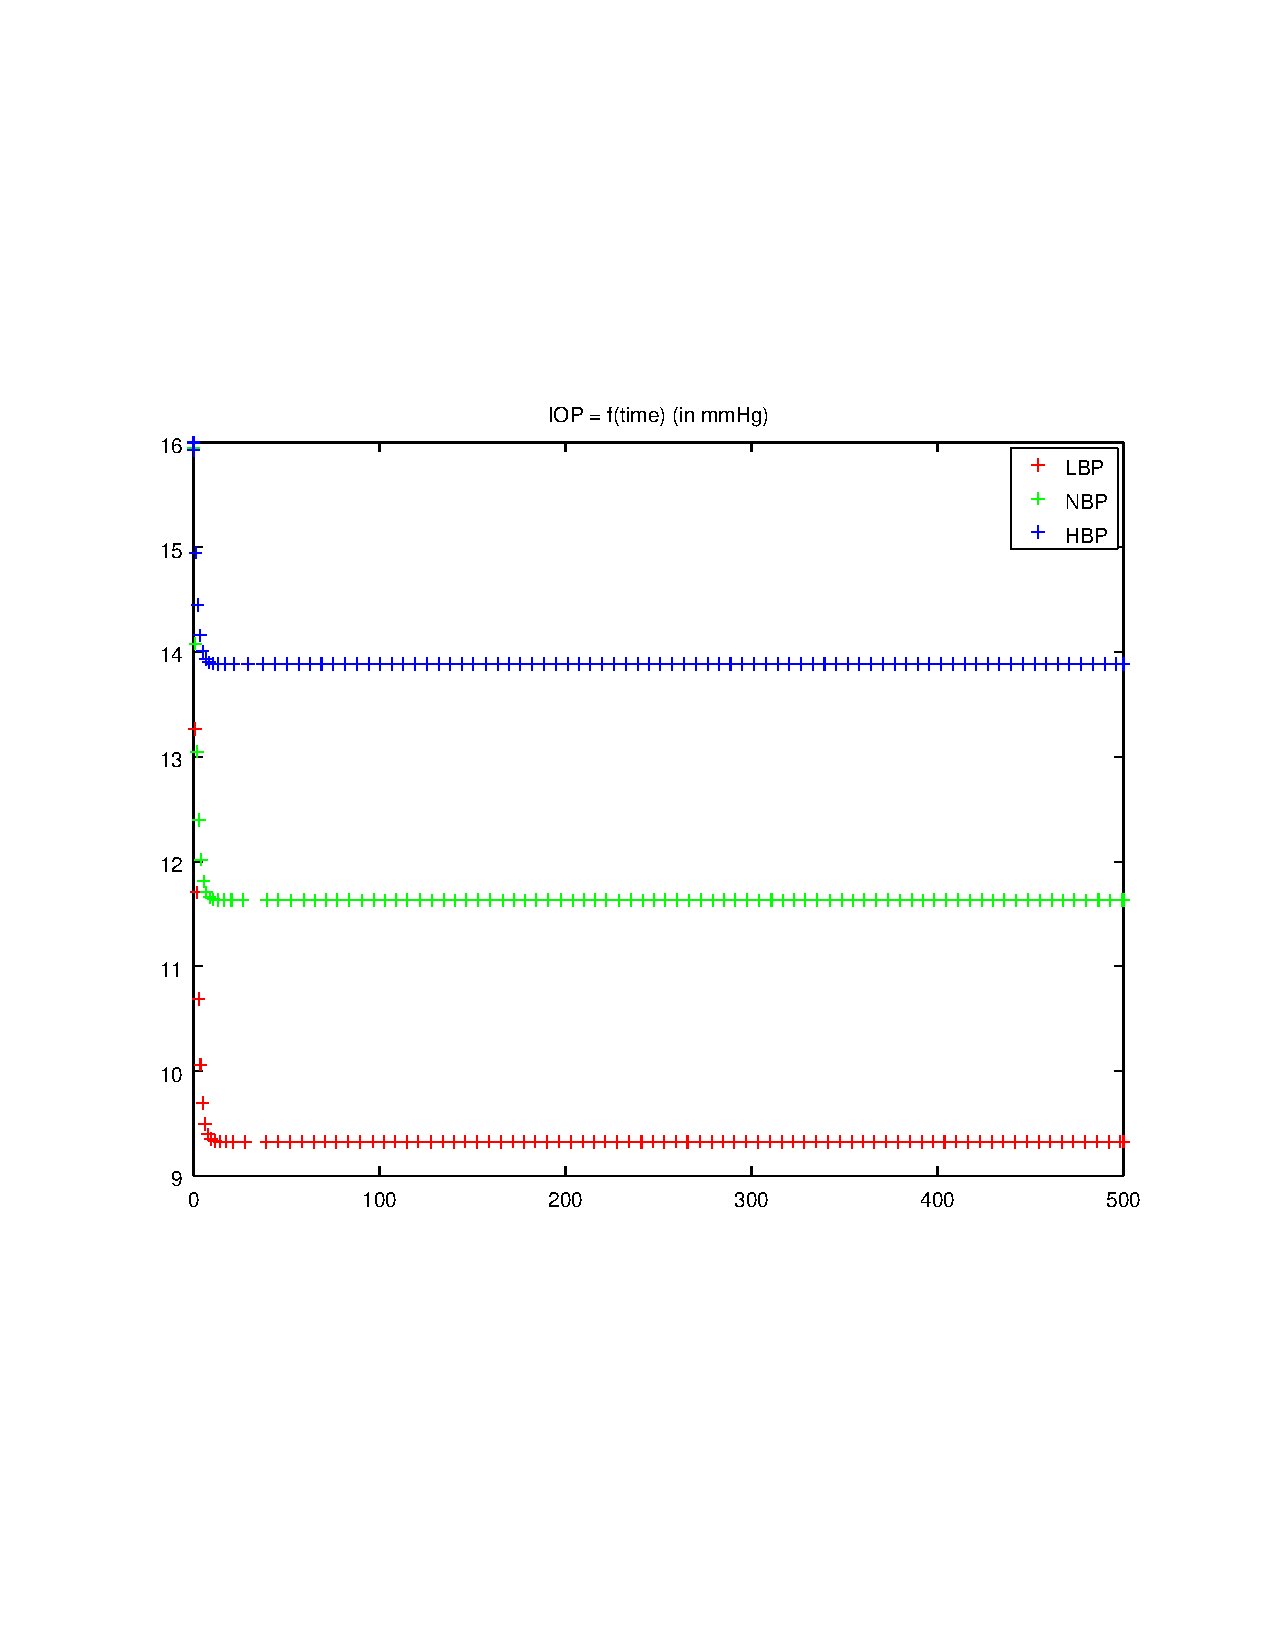
\includegraphics[width=0.45\textwidth]{images/IOP_time}
  }
  \subfigure[Time evolution of $C_2$\label{fig:C2t}]{
   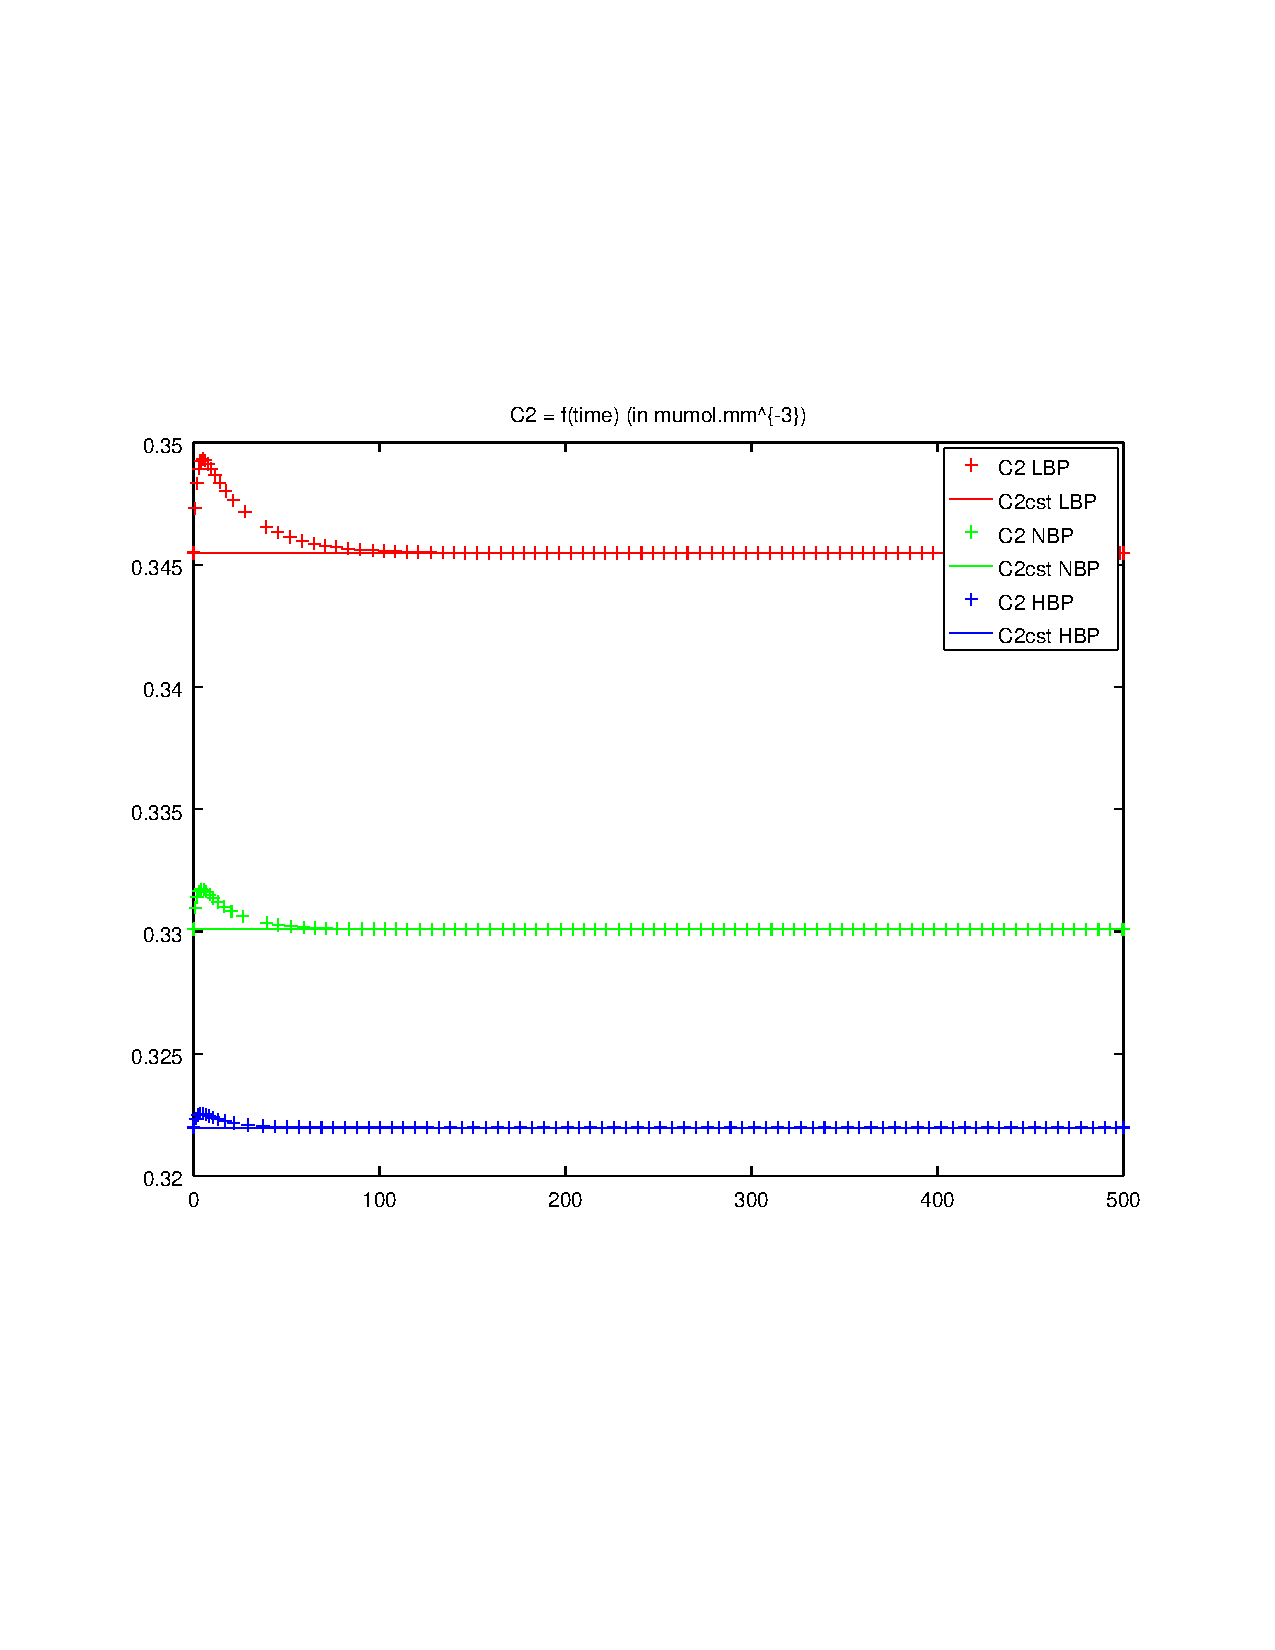
\includegraphics[width=0.45\textwidth]{images/C2_time}
 }
 
  \caption[text1]{Time evolution of IOP and $C_2$ }
    \label{fig:tevolpc2}
\end{figure}


\input 

\end{document}
